%!TEX root = ../Master.tex
\section{implementation details}\label{sec:impl}
This section presents a brief description of the three components of the system and how their implementation effect the system's behaviour and video playback delay.
\subsection{Transmission rate}
While the TxR sets the actual speed at which data is sent, it is not a direct measure of the amount of data, which can be transferred from the application layer over an extended period of time. We use throughput to denote the maintainable TxR. 802.11 utilize both packet headers and tails, which lower the throughput. Parts of the header is always transmitted at the lowest TxR for compatibility reasons. The largest contributor to why the throughput is lower than a selected data rate is the protocol behaviour. The protocol behaviour renders the channel idle for certain periods of time \cite{WorksheetThroughput,Throughput80211}. The usable throughput of 802.11 is the amount of payload it is able to service. This can be measured as the number of MAC layer service data units (SDU) transmitted over a period of time. An SDU is the payload a layer provides to the above layer. The MAC SDU can be seen on Figure \ref{fig:headers}.
\begin{figure}[ht]
  \centering
  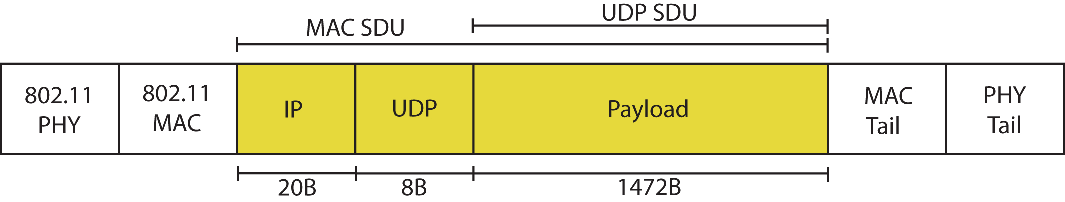
\includegraphics[width=\linewidth]{images/headers.pdf}
  \caption{802.11 frame with network interface, network and transport layer headers marked}
  \label{fig:headers}
\end{figure}

The protocol overhead also imposes limitations since the MAC SDU is limited to 1500 bytes (B) and IP \& UDP also require additional overhead. The IP header takes 20 B and has no protocol behaviour which impose further overhead. UDP takes an additional 8 B, leaving 1472 B of the MAC SDU throughput available to user applications.

Because 802.11 is a wireless communication technology the physical placement of the sender and receiver effect the performance. As the signal propagates the strength decreases with distance and reflections/interference can corrupt packets in transit. The different TxR described in 802.11 have different signal modulation which means the probability of packet corruption differs. By lowering the TxR, packets are less sensitive to noise and interference, therefore it is a trade-off between transmission speed and sensitivity.

\subsection{Random Linear Network Coding}
%In wireless communication transmission errors are imminent and if the MAC layer detects an error the packet is erased. Since packets are not retransmitted in 802.11 multicast an error results in data loss at the receivers. There are two techniques for minimizing losses: error correction which is the ability to detect and correct an error within a packet and erasure correction which is the ability to reobtain data after a erasure.

RLNC works by creating coded packets that are random linear combinations of a set of original packets called a generation. A generation consists of $n$ packets and can be used to generate an arbitrary amount of coded packets of size $n+k$, see Figure \ref{fig:NCIll}. $k$ is the number of redundant packet and can be varied such that it matches the packet loss in the channel. It is possible to obtain the original data if at least $n$ linearly independent packets are received.
\begin{figure}[ht]
	\centering
	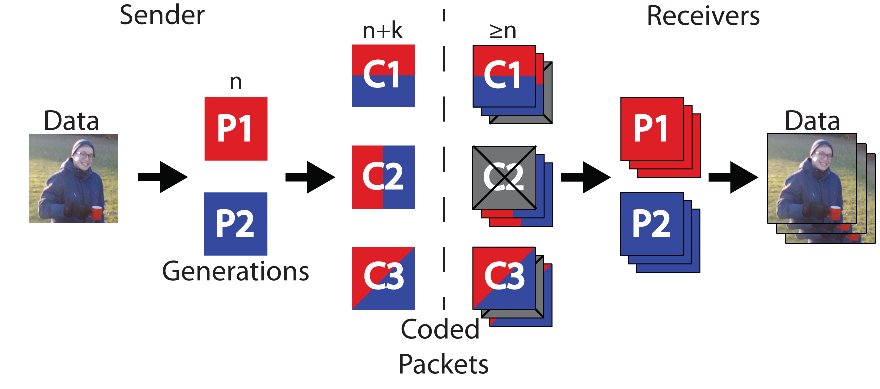
\includegraphics[width=\linewidth]{images/NetworkCoding.pdf}
	\caption{Usage of RLNC is showed, from coding (left) to decoding (right)}
	\label{fig:NCIll}
\end{figure}

RLNC is flexible since no prior information is needed at the receivers as each coded packet is self contained. This makes information sharing between the receivers easier. If a receiver has less than $n$ packets, it can reobtain its missing packet from another receiver. Therefore RLNC becomes advantageous compared to retransmissions when packet losses are uncorrelated, which is the case for our system\cite{WorksheetGrid,anime}.
These features come at a cost of an extra data and computational overhead when encoding and decoding which introduces additional system delay. Additionally, the randomness of the coding process can result in linear dependency between coded packets, which can result in situation where n packets are received but decoding is impossible.

\subsection{Video rate}
The video rate is the last resource we want to change to gain a reliable live video stream. The video quality should be as high as possible at all times given the application requirements. To change the video rate appropriately, an understanding of how the different parameters in H.264 work and how they affect the nature of the data stream \cite{WorksheetH264}.
H.264 consist of I, P and B frames, where only the I and P frame are used for streaming. The I-frame consists of the whole image and is needed when receivers join the stream. A P-frame is the difference in the picture from a previous P-frame or an I-frame.
For controlling the bit rate we use variable bitrate (VBR), which allocates as much data needed to every frame. In order to restrain the data size, a target bitrate is specified, which the encoder aims to achieve on average \cite{WorksheetH264}. The bitrate is highly dependent on the change in the video, which can be unpredictable. Because only the necessary data is allocated for each frame the bandwidth is used efficiently.
